\documentclass[conference]{IEEEtran}
\IEEEoverridecommandlockouts
\usepackage[T1]{fontenc}
\usepackage[utf8]{inputenc}
\usepackage{cite}
\usepackage{amsmath,amssymb}
\usepackage{graphicx}
\usepackage{booktabs,array}
\usepackage{xcolor}
\usepackage{soul}
\sethlcolor{yellow}
\usepackage{url}
\usepackage[hidelinks]{hyperref}
\newlength{\tabw}
\def\BibTeX{{\rm B\kern-.05em{\sc i\kern-.025em b}\kern-.08em T\kern-.1667em\lower.7ex\hbox{E}\kern-.125emX}}
\begin{document}
\title{PyGeoVision and PyGeoFetch: An Open Python Stack That Turns a Bounding Box into an Auditable Earth-Observation Deliverable, with Evidence from Fourteen Real Runs}
\author{\IEEEauthorblockN{Samuel Appiah Kubi}
\IEEEauthorblockA{\textit{EOCoreINT, Accra, Ghana}\\
\hl{[corresponding author e-mail]}}}
\maketitle
\begin{abstract}
Earth-observation analysis is slow to start and hard to trust: analysts search several archives by hand, prepare the imagery themselves, and receive maps that rarely say what supports them. This paper presents PyGeoVision, an open-source Python layer of 41 named analysis pipelines, and PyGeoFetch, the acquisition engine beneath it, which registers 22 data providers and adds federated search, a preflight gate, and resumable, checksum-verified downloads. Using only real data, we examine fourteen runs made with released versions 2.1.8 to 2.2.0 in seven countries and set them beside external references. Each run needed one to five arguments (median 2.5) and returned 10 to 17 files (median 13), including a report with its limitations; a documented Google Earth Engine flood workflow has 13 steps. The two multisensor flood runs fall in the windows of independently documented events (Accra, 29 June 2026; Rasuwa, Nepal, 26 August 2026), and their evidence classes show that 72\% and 90\% of the mapped flood rested on optical imagery alone. In a Mexico City radar-interferometry run, the PyGeoFetch preflight excluded 48 of 115 candidate scenes before download (about 360 GB, 42\% of the candidate volume), and a velocity range of $-$35.5 to $-$2.9 cm/yr is directionally consistent with a published peak of $-$39.1 cm/yr. In central London, a water mask at the default threshold captured 54\% of the water area of a land-cover product. No accuracy against ground truth is claimed, no running time was recorded, and the developer is also the evaluator.
\end{abstract}
\begin{IEEEkeywords}
Earth observation, open-source software, data acquisition, flood mapping, Sentinel-1, Sentinel-2, InSAR, reproducibility, evidence classes
\end{IEEEkeywords}
\section{Introduction}

Free Sentinel-1 radar and Sentinel-2 optical imagery cover the Earth every few days \cite{torres2012sentinel1,drusch2012sentinel2}, yet most of the time between a question and a usable map is spent before the first analysis: finding scenes across archives with different interfaces and credentials, downloading terabytes, masking cloud, and aligning grids. At the other end, a finished map seldom states what supports it. A flood map does not say that nine tenths of its area rests on one sensor, and a change map does not say that cloud hid most of the scene.

Two kinds of tool address parts of this. Hosted platforms remove the download: Google Earth Engine \cite{gorelick2017gee}, openEO \cite{schramm2021openeo} and the Open Data Cube \cite{lewis2017datacube} run the computation next to the archive. Access libraries unify search and download across catalogs: EODAG \cite{eodag2026}, pystac-client \cite{pystacclient2026} and sentinelsat \cite{sentinelsat2026}. Model libraries such as TorchGeo \cite{stewart2022torchgeo} and TerraTorch \cite{gomes2025terratorch} help to train networks. What is less common, in the sources we consulted, is a locally installed layer that goes from a bounding box to a finished deliverable in one call, with acquisition, preparation, analysis and a report whose limitations travel with the map.

PyGeoVision \cite{appiahkubi2026pygeovision} is such a layer, and PyGeoFetch \cite{appiahkubi2025pygeofetch} is the acquisition and processing engine under it. The software was written by the author of this paper, and the evidence below comes from his own runs. We therefore restrict the study to what can be checked without ground truth: real runs, the numbers printed in their reports, and external sources that exist independently of the software.

This paper asks four research questions.

\begin{itemize}
\item \textbf{RQ1 (workflow effort).} On real runs, how many arguments does the analyst give and how many files come back, and how does this compare with a documented reference workflow?
\item \textbf{RQ2 (acquisition layer).} What does PyGeoFetch contribute that can be verified in its source, how does it compare with documented access tools, and what does its preflight gate avoid on a real, data-intensive run?
\item \textbf{RQ3 (external agreement).} Do the real runs fall in independently documented events, or agree with published references and with a second product, and where do they differ?
\item \textbf{RQ4 (transparency).} Do the reports expose the limits of their own numbers, including when a run fails?
\end{itemize}

The thesis is that a layer which acquires, prepares, analyzes and reports in one call lowers the effort to a defensible first result, and that the reports it writes make the limits of that result visible, but that this is a claim about workflow and reporting, not about accuracy, which the data do not permit us to assess. The contributions are:

\begin{enumerate}
\item a description of the two-layer stack, with its data flow, its two refusal gates and its evidence-class flood logic (Section III);
\item a source-level verification of PyGeoFetch and a documentary comparison with three access tools (RQ2);
\item an analysis of fourteen real runs, twelve of which pass explicit screening criteria, with effort indicators and a documented comparator (RQ1);
\item comparisons with external sources: two documented flood events, a published snow-cover evaluation, a second land-cover product, and a published InSAR result for Mexico City (RQ3);
\item a failure that the reports did not flag, with the check that would have caught it (RQ4).
\end{enumerate}

Section II reviews related work, Section III describes the stack and the study protocol, Section IV answers each question, and Section V discusses the answers, the limits and future work.

\section{Related Work}

\subsection{Flood, Snow and Subsidence Mapping}

Radar flood mapping exploits the drop of backscatter over calm open water. Operational chains threshold the backscatter, often with a histogram method such as Otsu's \cite{otsu1979}, and detect change against a dry reference \cite{twele2016flood,uddin2019bangladesh}; for Ghana, unsupervised time-series ratios have been used, with the authors noting limited in-situ validation \cite{toffah2026ghana}. Optical methods use the normalized difference water index \cite{mcfeeters1996ndwi} and its modified form \cite{xu2006mndwi}. The two sensors fail differently: radar confuses wind-roughened water, smooth ground and radar shadow with floodwater and misses flooding among buildings or under vegetation, while optical imagery fails under cloud. Floodwater does not collect on high ground, so the height above the nearest drainage (HAND) \cite{nobre2011hand}, computed from a depression-filled model \cite{barnes2014priorityflood} with D8 routing \cite{ocallaghan1984d8}, gives a physical filter that needs no training data. For snow, the normalized difference snow index with a threshold of 0.4 is the basis of the MODIS snow product \cite{hall1995ndsi}, whose daily Collection 6 maps agreed with 665 climate stations in Austria at an overall accuracy above 97\% \cite{tong2020snow}. For land subsidence, Sentinel-1 interferometry over Mexico City from more than 300 scenes gave rates of up to $-$39.1 cm/yr in Iztapalapa \cite{cigna2021mexico}.

\subsection{Platforms, Libraries and Access Tools}

Planetary-scale platforms move the computation to the data: Google Earth Engine \cite{gorelick2017gee} with geemap \cite{wu2020geemap}, openEO \cite{schramm2021openeo}, and the Open Data Cube \cite{lewis2017datacube} as served for Africa by Digital Earth Africa \cite{digitalearthafrica}. In R, sits classifies image time series on data cubes \cite{simoes2021sits}. In Python, eo-learn defines patches and workflows \cite{sentinelhub2021eolearn}, TorchGeo supplies datasets and pretrained models \cite{stewart2022torchgeo,paszke2019pytorch}, TerraTorch fine-tunes foundation models \cite{gomes2025terratorch}, GeoAI joins imagery search to AI workflows \cite{wu2026geoai,wu2021leafmap,wu2023samgeo}, and pyroSAR processes Sentinel-1 data \cite{truckenbrodt2019pyrosar}. Catalogs are standardized by the SpatioTemporal Asset Catalog specification \cite{stac2021}. Access is served by EODAG, whose documentation lists more than 270 configured collections \cite{eodag2026}; by pystac-client, which searches STAC APIs \cite{pystacclient2026}; and by sentinelsat, which searches and downloads Sentinel products \cite{sentinelsat2026}.

\subsection{Gap}

In the sources consulted, hosted platforms solve scale but not local reporting, access libraries stop at the files, and model libraries start from prepared data. Published flood studies report accuracy against reference maps but say little about reporting validity at the point of use. The questions of this paper are whether a layer that spans acquisition to report lowers the effort, whether its acquisition engine does something the access tools do not describe, whether its real runs agree with the outside world, and whether its reports tell the reader when they should not be trusted.

\section{Methodology}

\subsection{The Two-Layer Stack}

PyGeoVision (version 2.1.8 for the catalogue described here; MIT license; Python 3.10 or later) offers one client and one command line over 41 named pipelines, of which 34 run without trained weights, 79 model-registry entries, an object-based analysis module, and a reporting layer. PyGeoFetch (version 2.6.3; MIT license) is the acquisition and processing engine; PyGeoVision calls it through a bridge, and both share one credential store. Fig. 1 shows the layers and Fig. 2 one run. A run is a single statement,

\begin{scriptsize}
\begin{verbatim}
result = client.pipeline("multisensor_flood_mapping",
    bbox=(-0.35, 5.45, 0.05, 5.75),
    date_before="2026-06-01/2026-06-20",
    date_after="2026-06-27/2026-07-06",
    output_dir="out/accra")
\end{verbatim}
\end{scriptsize}

or the equivalent command \texttt{pygeovision channel multisensor\_\allowbreak{}flood\_\allowbreak{}mapping}, with every other argument at its default. Two refusals are built in: a pipeline that needs a trained model stops before any download if none is given, and a scene with fewer than 5\% clear pixels is not used (up to three alternative scenes are tried). Cloud and shadow become no-data, never a class, and each run writes a report with its limitations and a machine-readable record, \texttt{run\_\allowbreak{}summary.json}.

\begin{figure*}[!t]
\centering
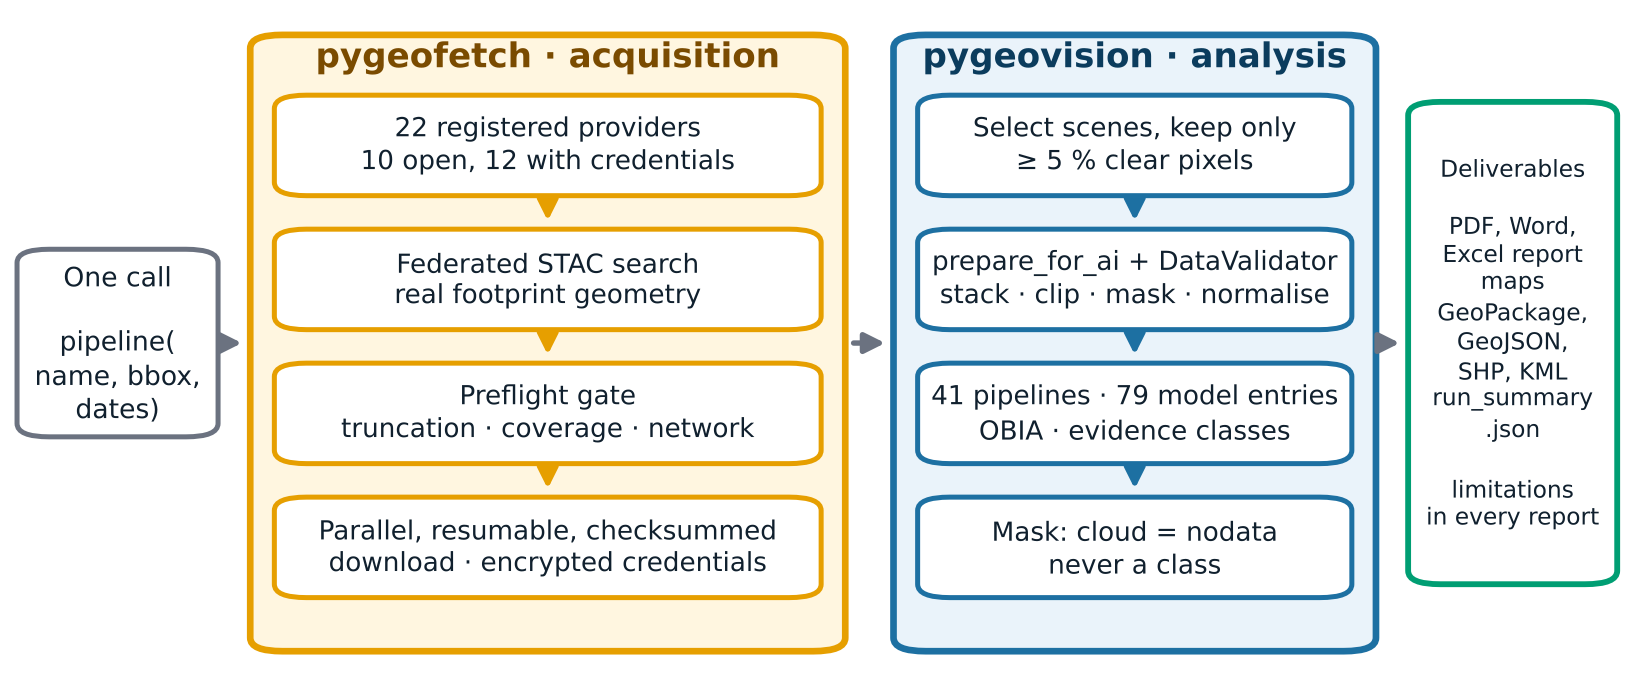
\includegraphics[width=\textwidth,height=9.2cm,keepaspectratio]{figs/fig_arch.png}
\caption{Two-layer architecture: PyGeoFetch acquires, PyGeoVision analyzes and reports. One call enters the acquisition layer (providers, federated search, preflight, checked download) and passes prepared data to the analysis layer, which writes the deliverables. PyGeoFetch counts are from its provider registry (22) as installed in version 2.6.3.}
\end{figure*}

\begin{figure*}[!t]
\centering
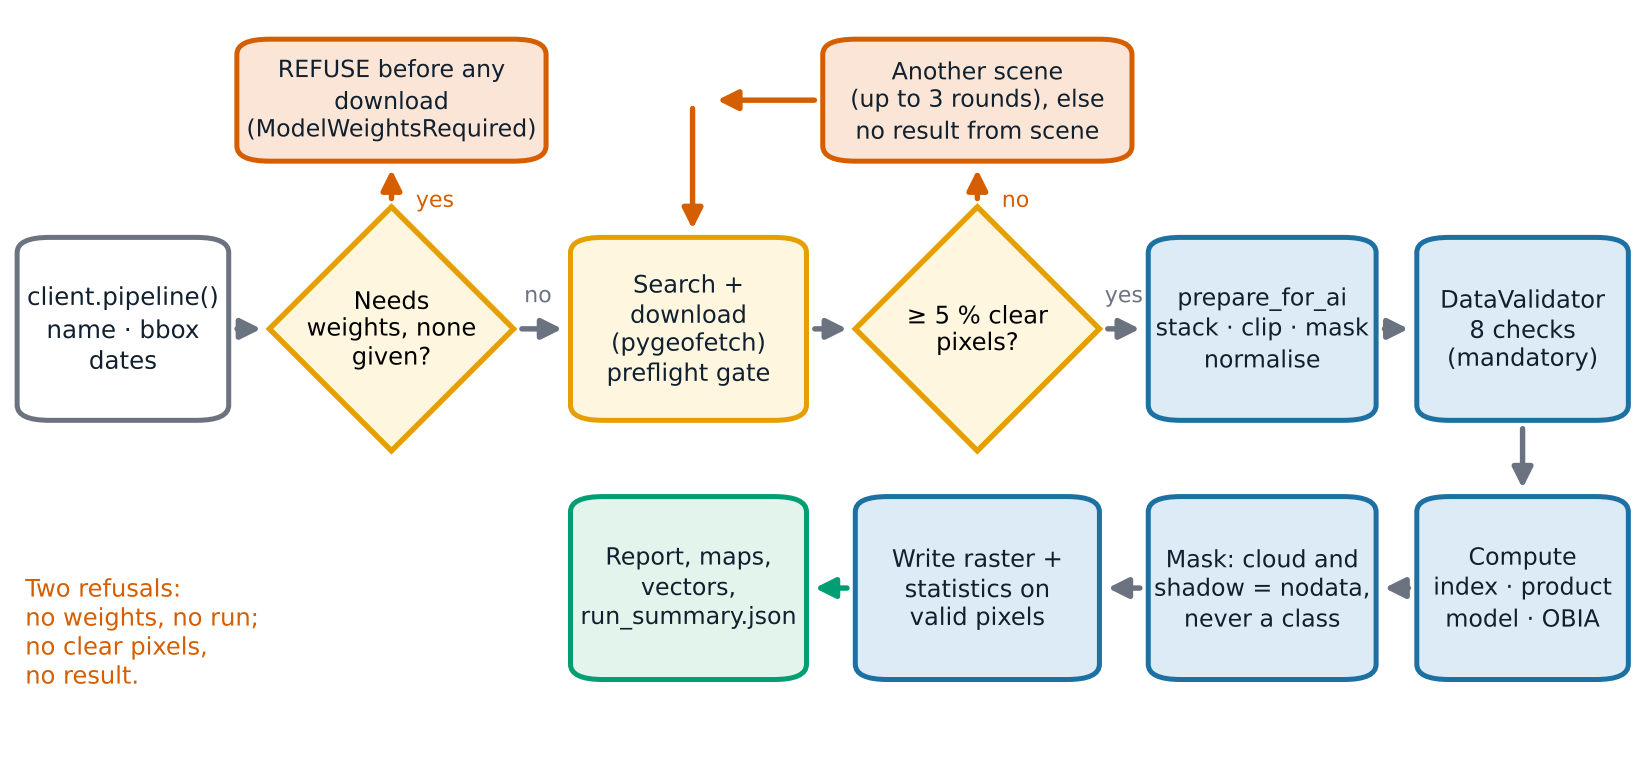
\includegraphics[width=\textwidth,height=9.2cm,keepaspectratio]{figs/fig_flow.png}
\caption{Data flow of one pipeline run with its two refusal gates. A pipeline that needs weights and has none stops before any download; a scene with fewer than 5\% clear pixels is replaced by another (up to three rounds). Cloud and shadow are written as no-data. Deliverables: report in three formats, maps, vector layers and the run record.}
\end{figure*}

\subsection{The Multisensor Flood Pipeline}

The pipeline compares a reference window R with a flood window F. The radar water threshold T$_{\mathrm{w}}$ is chosen so that radar water in R agrees best, in the F1 sense, with optical water in R; if the optical view is unusable, the conventional $-$15 dB is used and its source is recorded as a default. A pixel is a radar flood candidate when

\begin{equation}
F(x)=1\ \text{if}\ \sigma_{\mathrm{flood}}(x)<T_{\mathrm{w}},\ \sigma_{\mathrm{ref}}(x)\geq T_{\mathrm{w}},\ \Delta(x)\leq -3\ \mathrm{dB}
\end{equation}

where $\Delta$(x) is $\sigma$$_{\mathrm{F}}$(x) $-$ $\sigma$$_{\mathrm{R}}$(x) after the mean brightness offset between the windows is removed. Optical water is MNDWI > 0 \cite{xu2006mndwi},

\begin{equation}
\mathrm{MNDWI}=\frac{\rho_{\mathrm{green}}-\rho_{\mathrm{SWIR1}}}{\rho_{\mathrm{green}}+\rho_{\mathrm{SWIR1}}}
\end{equation}

computed from Sentinel-2 L2A bands, masked by the Scene Classification Layer and reduced to the median of the clear observations in each window. A cloudy pixel is unknown, never dry. Each pixel is assigned to one of five evidence classes (Fig. 3): 1 radar and optical agree, 2 radar only (no clear optical view), 3 optical only, 4 disputed (radar flooded, clear optical view dry), 5 water in the reference window. The flooded area is classes 1 to 3; an upper bound adds class 4. Where a terrain model is available, flooded pixels more than 15 m above the nearest drainage are removed,

\begin{equation}
\mathrm{HAND}(x)=z(x)-z\bigl(d(x)\bigr)
\end{equation}

where z is elevation and d(x) the drainage cell into which x drains \cite{nobre2011hand}. Patches smaller than 0.1 ha are removed. The terrain stage runs only on grids of at most six million cells, and the report says when it did not run.

\begin{figure}[!t]
\centering
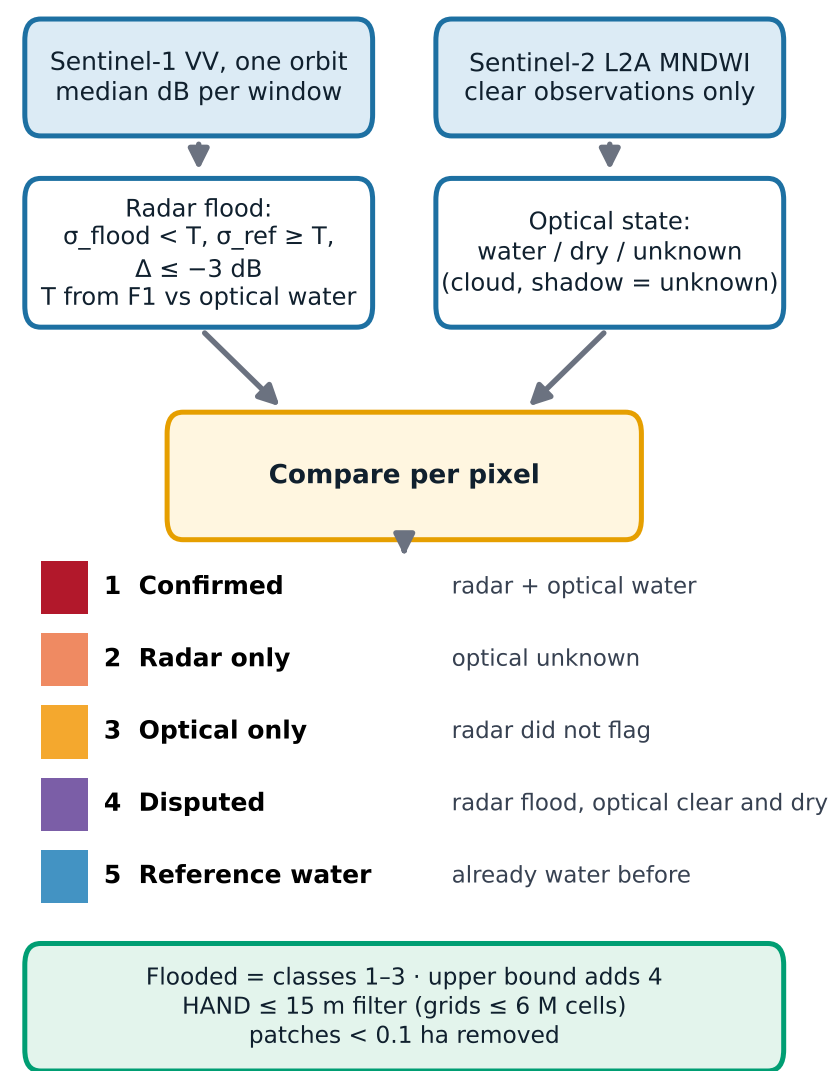
\includegraphics[width=\columnwidth,height=10.5cm,keepaspectratio]{figs/fig_evidence.png}
\caption{Evidence-class logic of the multisensor flood pipeline. Radar and optical evidence are kept apart and compared per pixel; the five classes, the three reported areas and the terrain filter follow.}
\end{figure}

\subsection{Study Protocol and Screening}

The study uses only real data. We examine every report that the author had produced with released versions of the software (14 reports, generated 10 to 15 October 2026; 10 with version 2.1.8, two with 2.1.9, two with 2.2.0) and give a pipeline name, place and result for each in Table I. Each report was read in full and its numbers were transcribed by hand. No run was repeated for this paper. A report passes screening if (C1) it was produced from real imagery or published products with a released version, (C2) its inputs are internally consistent (the two windows of a change analysis differ and the class areas add up), and (C3) the share of valid pixels is at least 40\%. Reports that fail are excluded from the results of RQ3 and reported in RQ4. The comparison with external sources uses only sources that we could read and that exist independently of the software; each was accessed on 19 or 20 October 2026.

\begin{table*}[!t]
\caption{The fourteen real reports and the screening result}
\centering
{\scriptsize\setlength{\tabcolsep}{2.5pt}\renewcommand{\arraystretch}{1.12}\setlength{\tabw}{\dimexpr\textwidth-14\tabcolsep\relax}
\begin{tabular}{>{\raggedright\arraybackslash}p{\dimexpr0.1300\tabw\relax}>{\raggedright\arraybackslash}p{\dimexpr0.1800\tabw\relax}>{\raggedright\arraybackslash}p{\dimexpr0.1400\tabw\relax}>{\raggedright\arraybackslash}p{\dimexpr0.0700\tabw\relax}>{\raggedright\arraybackslash}p{\dimexpr0.0900\tabw\relax}>{\raggedright\arraybackslash}p{\dimexpr0.1700\tabw\relax}>{\raggedright\arraybackslash}p{\dimexpr0.2200\tabw\relax}}
\toprule
\textbf{Run} & \textbf{Pipeline} & \textbf{Place} & \textbf{Version} & \textbf{Valid share} & \textbf{Screening} & \textbf{External anchor used} \\
\midrule
Flood, Accra & multisensor\_\allowbreak{}flood\_\allowbreak{}mapping & Greater Accra, Ghana & 2.1.8 & 100\% radar; 18.1\% optical & Included & Event of 29 June 2026 \cite{citi2026accra} \\
Flood, Nepal & multisensor\_\allowbreak{}flood\_\allowbreak{}mapping & Central Nepal & 2.1.8 & 100\% radar; 19.8\% optical & Included & Event of 26 August 2026 \cite{cems2026emsr927,nrsc2026trishuli} \\
Snow and ice & snow\_\allowbreak{}cover & Swiss Alps & 2.2.0 & 93.4\% & Included & MODIS method and station evaluation \cite{hall1995ndsi,tong2020snow} \\
Land cover & land\_\allowbreak{}cover & Central London & 2.1.8 & product & Included & Second product (water) \\
Surface water & water\_\allowbreak{}bodies & Central London & 2.1.8 & 98.2\% & Included & Land-cover product \\
Drainage and HAND & drainage\_\allowbreak{}analysis & Tyrol, Austria & 2.1.8 & 100\% & Included & Method \cite{nobre2011hand} \\
Burn severity & wildfire\_\allowbreak{}severity & Northern California & 2.1.8 & 95.9\% & Included & Class limits \cite{key2006firemon} \\
Buildings & building\_\allowbreak{}footprints & Central London & 2.1.8 & dataset & Included & None \\
Roads & road\_\allowbreak{}network & Central London & 2.1.8 & dataset & Included & None \\
Vegetation change & crop\_\allowbreak{}health & Central London & 2.2.0 & 44.2\% & Included (warning printed) & None \\
Habitat hotspots & biodiversity\_\allowbreak{}hotspot & Central London & 2.1.9 & product & Included & None \\
Evapotranspiration & evapotranspiration & South-east Ghana & 2.1.9 & 96.3\% & Included & None \\
Coastal change & coastal\_\allowbreak{}monitoring & Dutch coast & 2.1.8 & 1.7\% & Excluded (C3) & None \\
Flood, radar only & sar\_\allowbreak{}flood\_\allowbreak{}mapping & Greater Accra, Ghana & 2.1.8 & 100\% & Excluded (C2) & None \\
\bottomrule
\end{tabular}
\par\vspace{2pt}\begin{minipage}{\textwidth}\raggedright\scriptsize Note: ``product'' and ``dataset'' mean that the input is a published map or footprint dataset, for which a valid share is not defined. Twelve of fourteen runs pass screening.\end{minipage}
}
\end{table*}

\subsection{Effort Indicators and Documentary Comparator}

Effort is measured by two counts that every report prints: the arguments listed in its Pipeline table (box, dates and any non-default setting) and the files listed in its Deliverables table. Both are counts, not times; neither the running time nor the data volume of these runs was recorded. As a documented comparator for flood mapping we take the UN-SPIDER recommended practice for Sentinel-1 flood mapping in Google Earth Engine \cite{unspider2026flood}, counting its numbered steps and the auxiliary layers it names. The comparison is documentary: the two workflows differ in sensors, outputs and where the computation runs.

\subsection{Verification of the Acquisition Layer}

The capabilities of PyGeoFetch are verified in the installed package (version 2.6.3): the provider registry is called and counted, and the download manager, the credential store and the preflight gate are read in source. The documentation of EODAG, pystac-client and sentinelsat was read on the pages cited; a dash in Table IV means the pages read do not describe the feature, not that it is absent. The Mexico City run is taken from the project documentation of PyGeoFetch and from the companion case-study repository, which we read but did not re-run.

\subsection{Statistics}

Without ground truth, one run per case and no replicates, no accuracy or interval can be computed for the case-study results, and none is claimed. Proportions of reports are given with exact Clopper--Pearson intervals. Everything else is a count or an area transcribed from a report, with its source. The paired-bootstrap design used for controlled comparisons needs a reference that these runs do not have.

\subsection{Reproducibility and Disclosure}

The 14 reports and the PyGeoFetch registry listing are supplied with the manuscript; the software is public. The author used Claude (Anthropic) to read the reports, to check them against the repository, to verify references and to draft and restructure the text, and has reviewed the output and takes responsibility for it.

\begin{table*}[!t]
\caption{Inputs of the externally anchored runs}
\centering
{\footnotesize\setlength{\tabcolsep}{2.5pt}\renewcommand{\arraystretch}{1.12}\setlength{\tabw}{\dimexpr\textwidth-10\tabcolsep\relax}
\begin{tabular}{>{\raggedright\arraybackslash}p{\dimexpr0.1300\tabw\relax}>{\raggedright\arraybackslash}p{\dimexpr0.1900\tabw\relax}>{\raggedright\arraybackslash}p{\dimexpr0.1200\tabw\relax}>{\raggedright\arraybackslash}p{\dimexpr0.2500\tabw\relax}>{\raggedright\arraybackslash}p{\dimexpr0.3100\tabw\relax}}
\toprule
\textbf{Run} & \textbf{Box (west, south, east, north)} & \textbf{Area} & \textbf{Dates} & \textbf{Inputs actually used} \\
\midrule
Flood, Accra & $-$0.35, 5.45, 0.05, 5.75 & 1,470 km$^{2}$ & Reference 1--20 Jun; flood 27 Jun--6 Jul 2026 (scenes 2--9 Jun and 27 Jun--3 Jul) & Sentinel-1 RTC VV, ascending, orbit 147 (3 + 2 scenes); Sentinel-2 L2A (10 + 6); Copernicus 30 m DEM \\
Flood, Nepal & 84.8, 27.7, 85.6, 28.3 & 5,232 km$^{2}$ & Reference 10--24 Aug; flood 26--28 Aug 2026 & Sentinel-1 RTC VV, ascending, orbit 85 (2 + 2); Sentinel-2 L2A (10 + 1); no terrain stage \\
Snow and ice & 7.8, 46.4, 8.2, 46.7 & 1,023 km$^{2}$ & January 2024 & One Sentinel-2 L2A scene (11 Jan 2024) \\
Land cover; surface water & $-$0.15, 51.47, $-$0.10, 51.52 & 19.3 km$^{2}$ & WorldCover 2021; June 2024 & ESA WorldCover 10 m; one Sentinel-2 L2A scene (26 Jun 2024) \\
InSAR, Mexico City & $-$99.183, 19.278, $-$99.003, 19.438 & about 335 km$^{2}$ & July 2016--September 2017 & Sentinel-1 SLC (67 downloaded); SRTM 30 m DEM \\
\bottomrule
\end{tabular}
\par\vspace{2pt}\begin{minipage}{\textwidth}\raggedright\scriptsize Note: The area of the Mexico City box is computed from its corners. Scene counts are from the reports (flood runs) and from the project documentation (Mexico City).\end{minipage}
}
\end{table*}

\section{Results}

\subsection{RQ1: Workflow Effort}

Across the fourteen reports the analyst listed one to five arguments (median 2.5; Fig. 4a) and each run returned 10 to 17 files (median 13; Fig. 4b): the report in PDF, Word and Excel, maps, vector layers and the run record. Restricting to the twelve screened runs gives the same medians. The two multisensor flood runs listed three arguments, the box and two windows, and returned 17 and 15 files. The highest count of arguments, five, belongs to the vegetation run (two dates, a cloud mask and an anomaly threshold). All runs used a single statement or command; the Python statement is shown in Section III-A.

\begin{figure*}[!t]
\centering
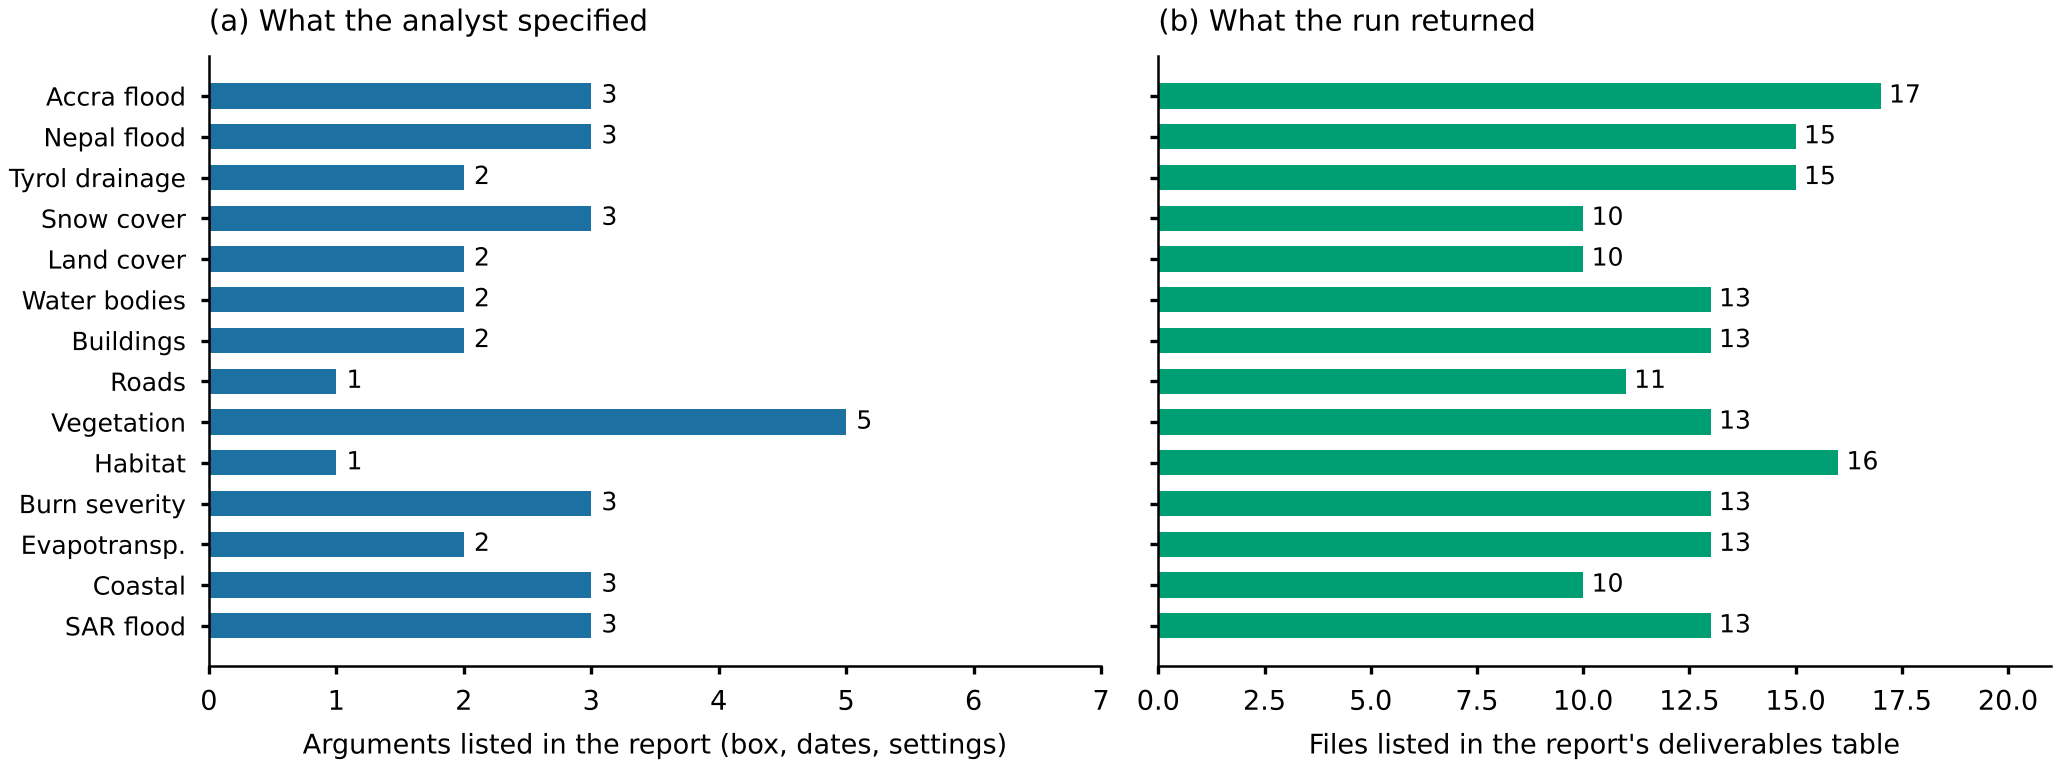
\includegraphics[width=\textwidth,height=9.2cm,keepaspectratio]{figs/fig_effort.png}
\caption{Effort indicators of the fourteen real runs. (a) Arguments listed in the report's Pipeline table. (b) Files listed in its Deliverables table. Both are counts transcribed from the reports; neither running time nor data volume was recorded.}
\end{figure*}

Table III sets the Accra run beside the UN-SPIDER recommended practice for flood mapping in Google Earth Engine \cite{unspider2026flood}, which has 13 numbered steps and names five auxiliary layers (country boundaries, JRC surface water, HydroSHEDS terrain, a population grid and a land-cover product). The comparison is indicative. The Earth Engine practice needs no download and adds exposed population, cropland and urban area, which the PyGeoVision pipeline does not. The PyGeoVision pipeline uses two sensors and a terrain filter, asks for three arguments, and returns a per-pixel evidence class and a report, but it moves scenes to the local machine.

\begin{table*}[!t]
\caption{Documented workflow: PyGeoVision flood run beside the UN-SPIDER Earth Engine practice}
\centering
{\footnotesize\setlength{\tabcolsep}{2.5pt}\renewcommand{\arraystretch}{1.12}\setlength{\tabw}{\dimexpr\textwidth-6\tabcolsep\relax}
\begin{tabular}{>{\raggedright\arraybackslash}p{\dimexpr0.2000\tabw\relax}>{\raggedright\arraybackslash}p{\dimexpr0.4000\tabw\relax}>{\raggedright\arraybackslash}p{\dimexpr0.4000\tabw\relax}}
\toprule
\textbf{Item} & \textbf{PyGeoVision multisensor flood (Accra run)} & \textbf{UN-SPIDER recommended practice \cite{unspider2026flood}} \\
\midrule
User-facing steps & One statement or command & 13 numbered steps \\
Arguments set & 3 (box, reference window, flood window) & Study area, time frame and sensor parameters (steps 1 and 2) \\
Sensors & Sentinel-1 RTC and Sentinel-2 L2A & Sentinel-1 GRD only \\
Auxiliary layers & Copernicus 30 m DEM fetched by the pipeline & Five named layers (boundaries, JRC water, HydroSHEDS, GHSL, MCD12Q1) \\
Where it runs & Local machine; scenes downloaded through PyGeoFetch & Google's hosted platform; no download \\
Terrain filter & HAND $\leq$ 15 m, reported as applied or skipped & Slope above 5\% removed \\
Evidence per pixel & Five classes (sensor agreement) & Single flood mask \\
Exposure outputs & None & Population, cropland, urban area \\
Files returned & 17, including a report with limitations & Exports chosen by the user \\
\bottomrule
\end{tabular}
\par\vspace{2pt}\begin{minipage}{\textwidth}\raggedright\scriptsize Note: The two workflows differ in scope and platform; the counts are documentary and not a benchmark. Running time was not measured for either.\end{minipage}
}
\end{table*}

\subsection{RQ2: PyGeoFetch}

\textit{Verified capabilities.} Calling the provider registry of the installed package returns 22 providers: 10 flagged as not requiring credentials (among them Planetary Computer, AWS Earth, Element84, NOAA Big Data and JAXA Earth) and 12 with credentials (Copernicus, USGS, NASA Earthdata and its cloud variant, Sentinel Hub, Planet, Maxar, Airbus, OpenTopography, Earth Explorer, Google Earth Engine, ISRO Bhuvan). In source, the download manager runs a configurable number of parallel workers, offers a resume option that skips files already present, verifies MD5 or SHA-256 checksums against provider values, and retries with back-off; credentials are held in the system keyring with an encrypted-file fallback; and a preflight gate checks search truncation, area coverage, temporal connectivity of the scene network and burst-timing compatibility before any download. The package also holds a preprocessing and spectral-index engine and a modular SAR and InSAR chain (coregistration, deburst, enhanced spectral diversity, flat-earth, atmospheric and ionospheric correction, unwrapping, time-series inversion). We read this code and called the registry; we did not run downloads.

\begin{table*}[!t]
\caption{Acquisition tools as described in the sources read}
\centering
{\scriptsize\setlength{\tabcolsep}{2.5pt}\renewcommand{\arraystretch}{1.12}\setlength{\tabw}{\dimexpr\textwidth-12\tabcolsep\relax}
\begin{tabular}{>{\raggedright\arraybackslash}p{\dimexpr0.1200\tabw\relax}>{\raggedright\arraybackslash}p{\dimexpr0.2000\tabw\relax}>{\raggedright\arraybackslash}p{\dimexpr0.1700\tabw\relax}>{\raggedright\arraybackslash}p{\dimexpr0.1700\tabw\relax}>{\raggedright\arraybackslash}p{\dimexpr0.1700\tabw\relax}>{\raggedright\arraybackslash}p{\dimexpr0.1700\tabw\relax}}
\toprule
\textbf{Tool} & \textbf{Documented scope} & \textbf{Providers or catalogs} & \textbf{Download} & \textbf{Pre-download screening} & \textbf{Processing} \\
\midrule
PyGeoFetch (source, version 2.6.3) & Access and processing, one API and command line & 22 registered providers & Parallel; resume option; MD5 or SHA-256 check; retries & Preflight gate: truncation, coverage, network, burst timing & Preprocessing, indices, SAR and InSAR chain \\
EODAG \cite{eodag2026} & Earth observation data access gateway & More than 270 collections; Copernicus, USGS, Planetary Computer, AWS and others & --- & --- & --- \\
pystac-client \cite{pystacclient2026} & Search of STAC catalogs and APIs & STAC APIs & --- & AOI coverage of an item (tutorial) & --- \\
sentinelsat \cite{sentinelsat2026} & Search and download of Sentinel products & The Copernicus Open Access Hub is named & download\_\allowbreak{}all in examples & --- & --- \\
\bottomrule
\end{tabular}
\par\vspace{2pt}\begin{minipage}{\textwidth}\raggedright\scriptsize Note: A dash means the pages read do not describe the feature; it does not mean the feature is absent. The three documentation sites were read on 20 October 2026.\end{minipage}
}
\end{table*}

\textit{A real run.} The Mexico City case study of PyGeoFetch (Sentinel-1 SLC, July 2016 to September 2017, Iztapalapa) is the data-intensive test. According to the project documentation, a search returned 115 candidate scenes (after the search limit was widened), the preflight gate excluded 48 of them before any download, and 67 validated scenes of about 7.5 GB each (about 502 GB) were downloaded; the 48 scenes not downloaded correspond to about 360 GB, or 42\% of the candidate volume (Fig. 5a, 5b). The 2,211 theoretically possible pairs of the 67 scenes were reduced by orbit-based pre-filtering and coregistration to 78 interferograms. After unwrapping, the 58-date network split into 17 disconnected islands, and the inversion used the largest (10 dates, 11 pairs). The 2nd to 98th percentile of vertical velocity over reliable pixels, about 0.2\% of the scene, was $-$35.5 to $-$2.9 cm/yr. The published peak for Iztapalapa is $-$39.1 cm/yr, from more than 300 scenes between 2014 and 2020 \cite{cigna2021mexico}. The two figures have the same sign and order of magnitude; they are different statistics from very different data volumes, and the project documentation itself calls the result directionally consistent and not a replication. It also lists unresolved inconsistencies (58 against 67 dates, an earlier 29-date subset, and the denominator of 406 pairs at one stage) and replaces an earlier figure of 1,200 GB for the avoided volume with 360 GB.

\begin{figure*}[!t]
\centering
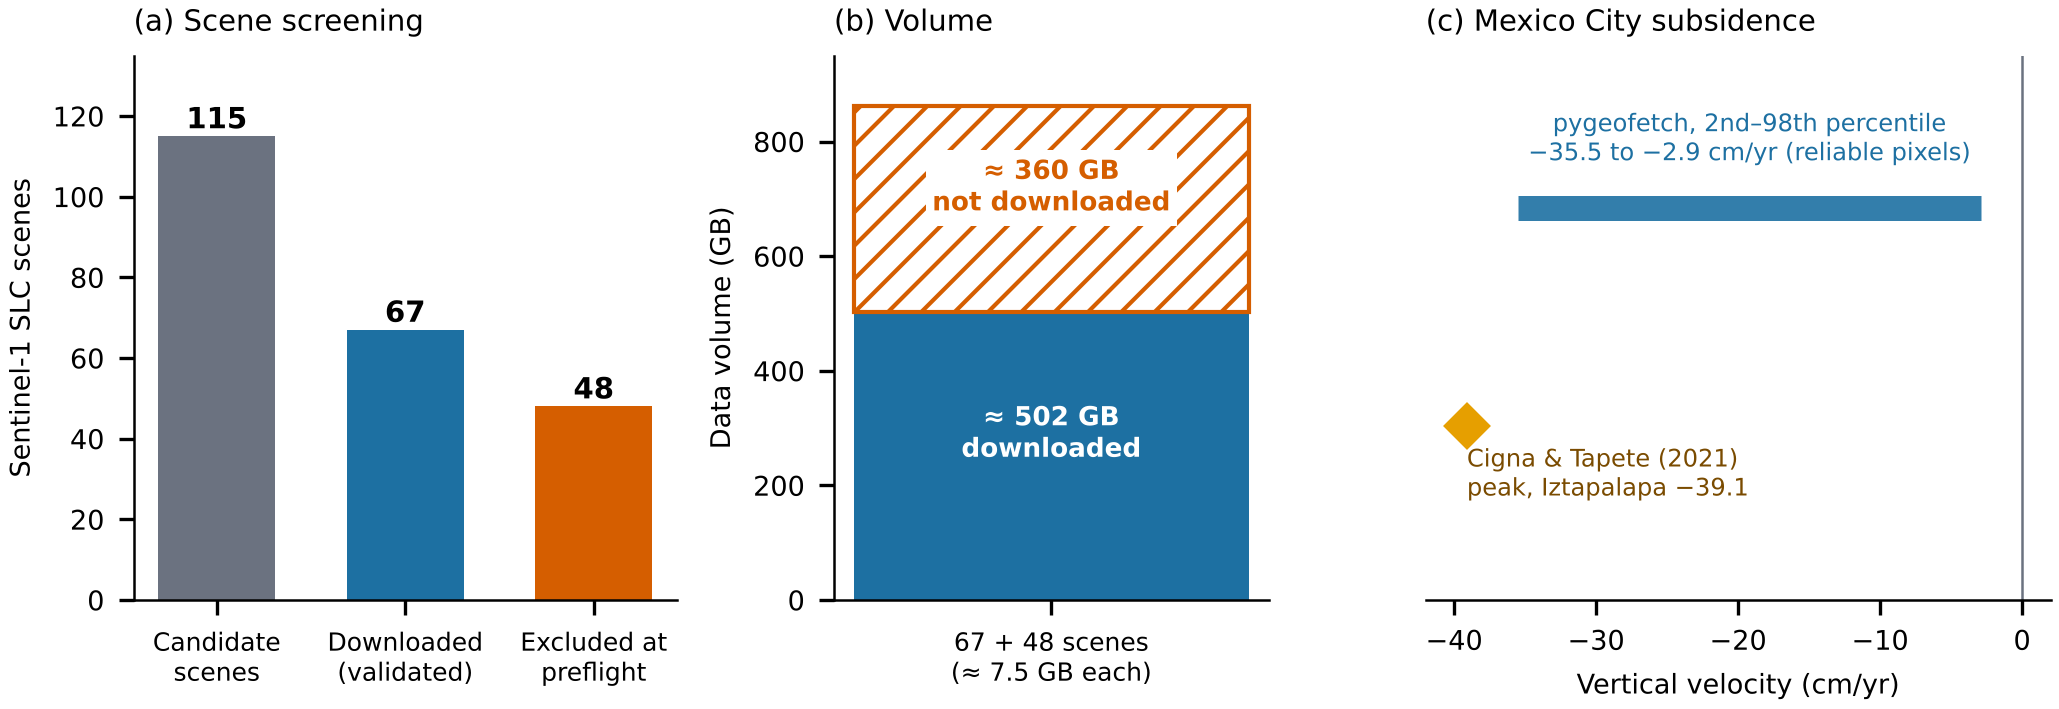
\includegraphics[width=\textwidth,height=9.2cm,keepaspectratio]{figs/fig_pgf.png}
\caption{PyGeoFetch on a real InSAR run: screening and agreement. (a) Sentinel-1 SLC scenes: candidates, downloaded, and excluded by the preflight gate. (b) Data volume, downloaded and not downloaded. (c) Vertical velocity range of the PyGeoFetch run (2nd--98th percentile over reliable pixels) beside the peak published for Iztapalapa \cite{cigna2021mexico}. Numbers are from the PyGeoFetch project documentation and were not re-run.}
\end{figure*}

The answer to RQ2 is that the source confirms 22 registered providers and the screening, checking and resuming features that the documentation claims, that the three access tools describe in the pages read only some of them, and that on one real run the gate kept 42\% of the candidate volume off the network. This is evidence of a feature working in one run, not a measured speed-up, and the figures come from the author's own project.

\subsection{RQ3: External Agreement}

Table V lists each externally anchored run beside what we could find outside the software.

\begin{table*}[!t]
\caption{Externally anchored runs: what the software reported and what exists outside it}
\centering
{\footnotesize\setlength{\tabcolsep}{2.5pt}\renewcommand{\arraystretch}{1.12}\setlength{\tabw}{\dimexpr\textwidth-8\tabcolsep\relax}
\begin{tabular}{>{\raggedright\arraybackslash}p{\dimexpr0.1200\tabw\relax}>{\raggedright\arraybackslash}p{\dimexpr0.2800\tabw\relax}>{\raggedright\arraybackslash}p{\dimexpr0.3800\tabw\relax}>{\raggedright\arraybackslash}p{\dimexpr0.2200\tabw\relax}}
\toprule
\textbf{Run} & \textbf{What PyGeoVision reported} & \textbf{External source} & \textbf{Agreement} \\
\midrule
Flood, Accra & 81.4 ha flooded (upper bound 84.8 ha), 0.1\% of land; 4.2 ha confirmed by both sensors; flood window 27 Jun--3 Jul & Flooding in Accra on Monday 29 June 2026; NADMO confirmed 10 deaths \cite{citi2026accra} & Event inside the window; no extent product found \\
Flood, Nepal & 451.7 ha flooded (upper bound 466.1 ha); 90\% optical only; flood window 26--28 Aug & Flash flood in Rasuwa on 26 August 2026, reportedly a glacial lake outburst, with a 7 m water level; rapid mapping requested (EMSR927) \cite{cems2026emsr927}; downstream districts Rasuwa, Dhading, Nuwakot, Gorkha, Chitwan \cite{nrsc2026trishuli}; about 100 km of runout \cite{roy2026nepalfloods} & Event inside the window; no area published in the pages read \\
Snow and ice & 93,272 ha snow or ice, 97.6\% of the valid area; NDSI > 0.40; valid share 93.4\%; one scene & Same threshold as the MODIS product \cite{hall1995ndsi}; daily MODIS maps agreed with 665 stations at 97.4--97.6\% \cite{tong2020snow} & Method agrees; no station check for this scene \\
Land cover and water, London & Water 124.7 ha (WorldCover 2021) against 66.9 ha (NDWI > 0.3, June 2024) in one box & The report notes that 0.3 is conservative and that the original cut is 0 \cite{mcfeeters1996ndwi} & Products differ by 46\%; threshold not varied \\
InSAR, Mexico City & $-$35.5 to $-$2.9 cm/yr (2nd--98th percentile) & Peak $-$39.1 cm/yr \cite{cigna2021mexico} & Directionally consistent \\
\bottomrule
\end{tabular}
\par\vspace{2pt}\begin{minipage}{\textwidth}\raggedright\scriptsize Note: Agreement is temporal or directional; it is not an accuracy assessment. Event sources were read on 20 October 2026.\end{minipage}
}
\end{table*}

\textit{Flood events.} Both multisensor runs bracket a documented event. The Accra windows (reference 2--9 June, flood 27 June to 3 July) contain the flooding of 29 June, and the Nepal windows (reference 10--24 August, flood 26--28 August) contain the flash flood of 26 August in Rasuwa, a district that the box overlaps together with Nuwakot and Dhading, which an Indian space agency charter map also names as affected. The evidence classes then say what the two sensors saw (Fig. 6, Fig. 7). In the Accra run only 4.2 ha (5\%) of 81.4 ha were seen by both sensors, 18.9 ha by radar alone and 58.2 ha (72\%) by optical alone, and optical imagery was clear over 18.1\% of the land. In the Nepal run 407.1 ha (90\%) of 451.7 ha were optical only and 13.2 ha (3\%) were confirmed; the terrain stage did not run because the grid held 13.5 million cells against a limit of six million; the radar threshold was the conventional $-$15.0 dB, a default whose source the report prints beside the scene's own Otsu value of $-$7.1 dB; and the flood window held a single optical scene against ten in the reference window. Of the radar-flagged pixels that a clear optical view could check, 105 of 191 (55\%) were confirmed in Accra and 329 of 689 (48\%) in Nepal. We found no published flood extent for either event in the sources read, so no area comparison is possible. Literature accuracies for radar flood maps, 94.0--96.1\% \cite{twele2016flood} and 96.44\% \cite{uddin2019bangladesh}, were measured against reference maps; the runs here had none. The Rasuwa event is, however, well documented: high-resolution post-event imagery of 27 and 28 August exists under an open license \cite{roy2026nepalfloods}, so the Nepal run can be validated.

\begin{figure*}[!t]
\centering
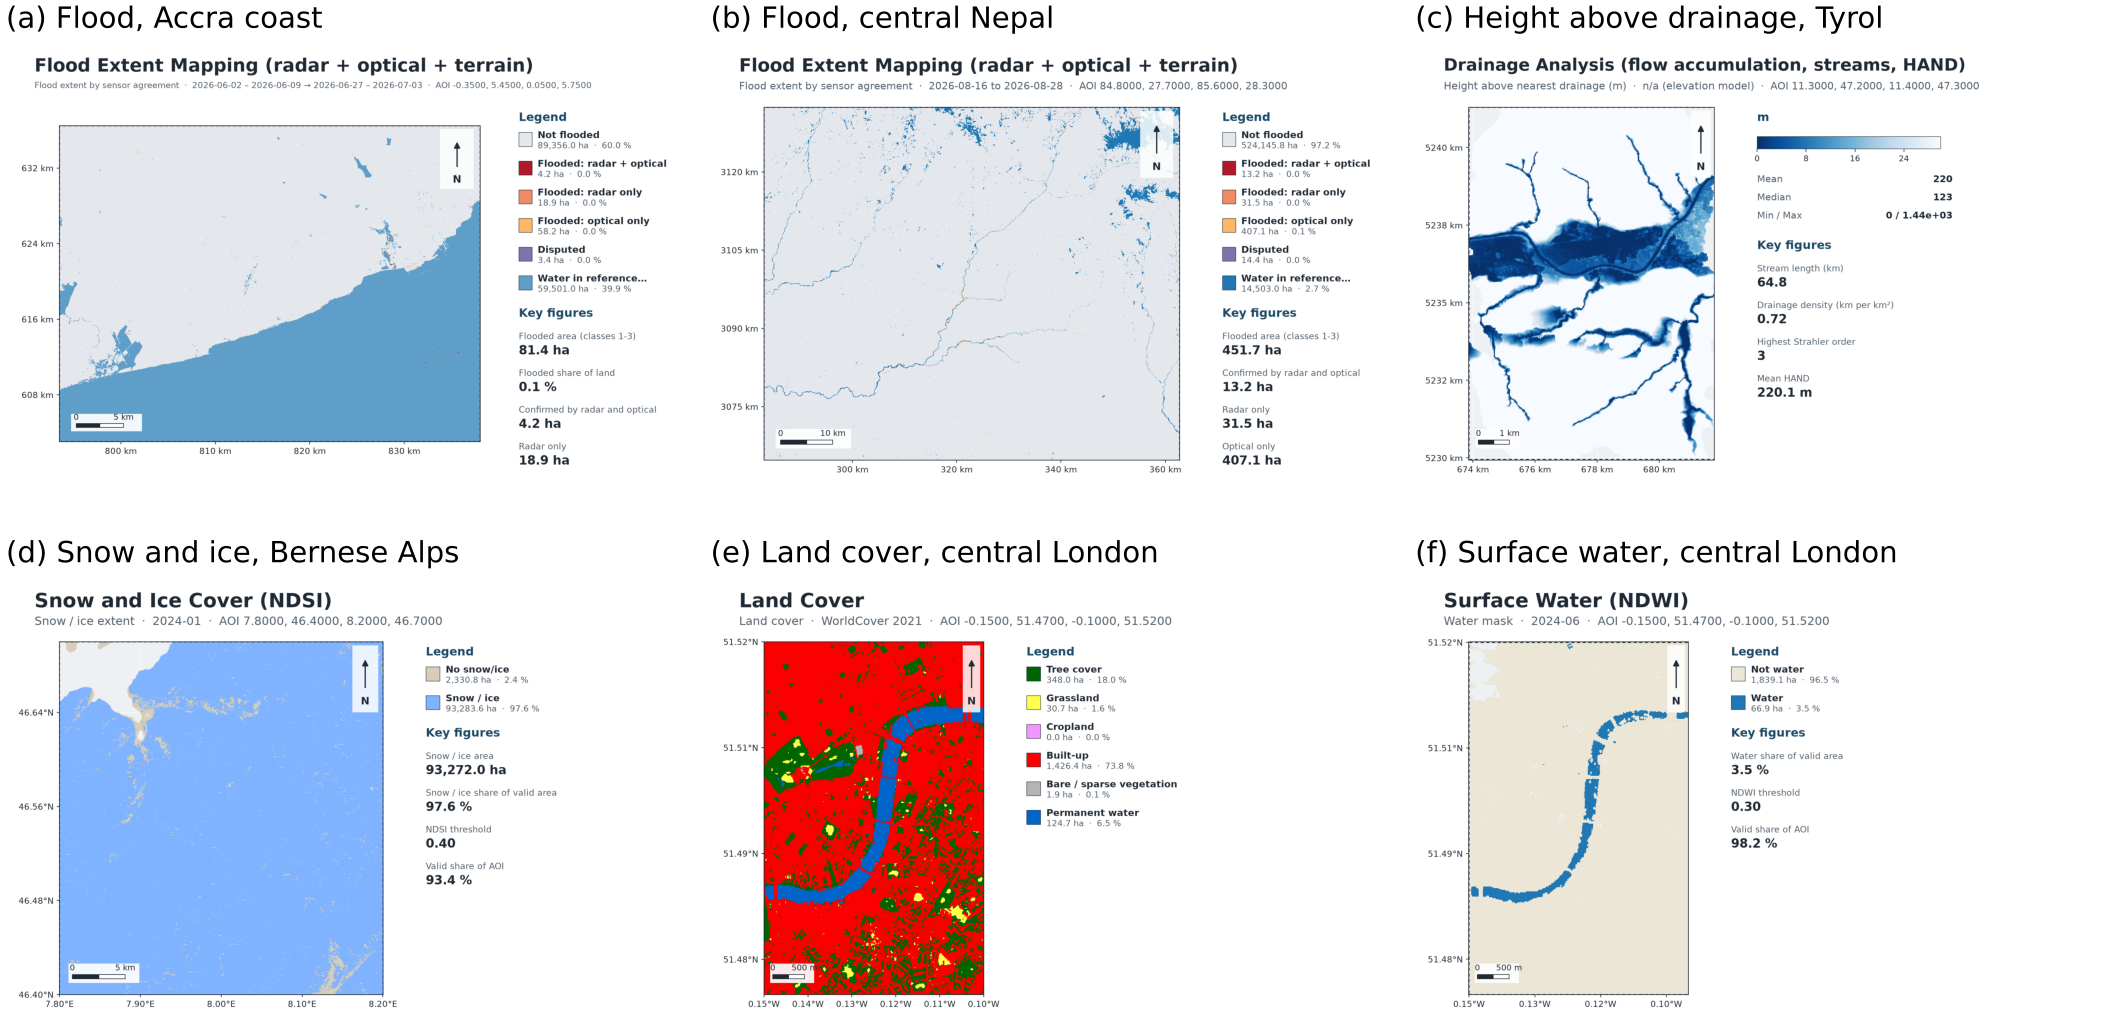
\includegraphics[width=\textwidth,height=9.2cm,keepaspectratio]{figs/fig_gallery.png}
\caption{Report maps of real runs. (a) Accra coast and (b) central Nepal: flood extent by sensor agreement. (c) Height above the nearest drainage, Tyrol. (d) Snow and ice, Swiss Alps. (e) Land cover and (f) surface water, central London. Maps are reproduced from the reports with their scale bars, north arrows and legends.}
\end{figure*}

\begin{figure*}[!t]
\centering
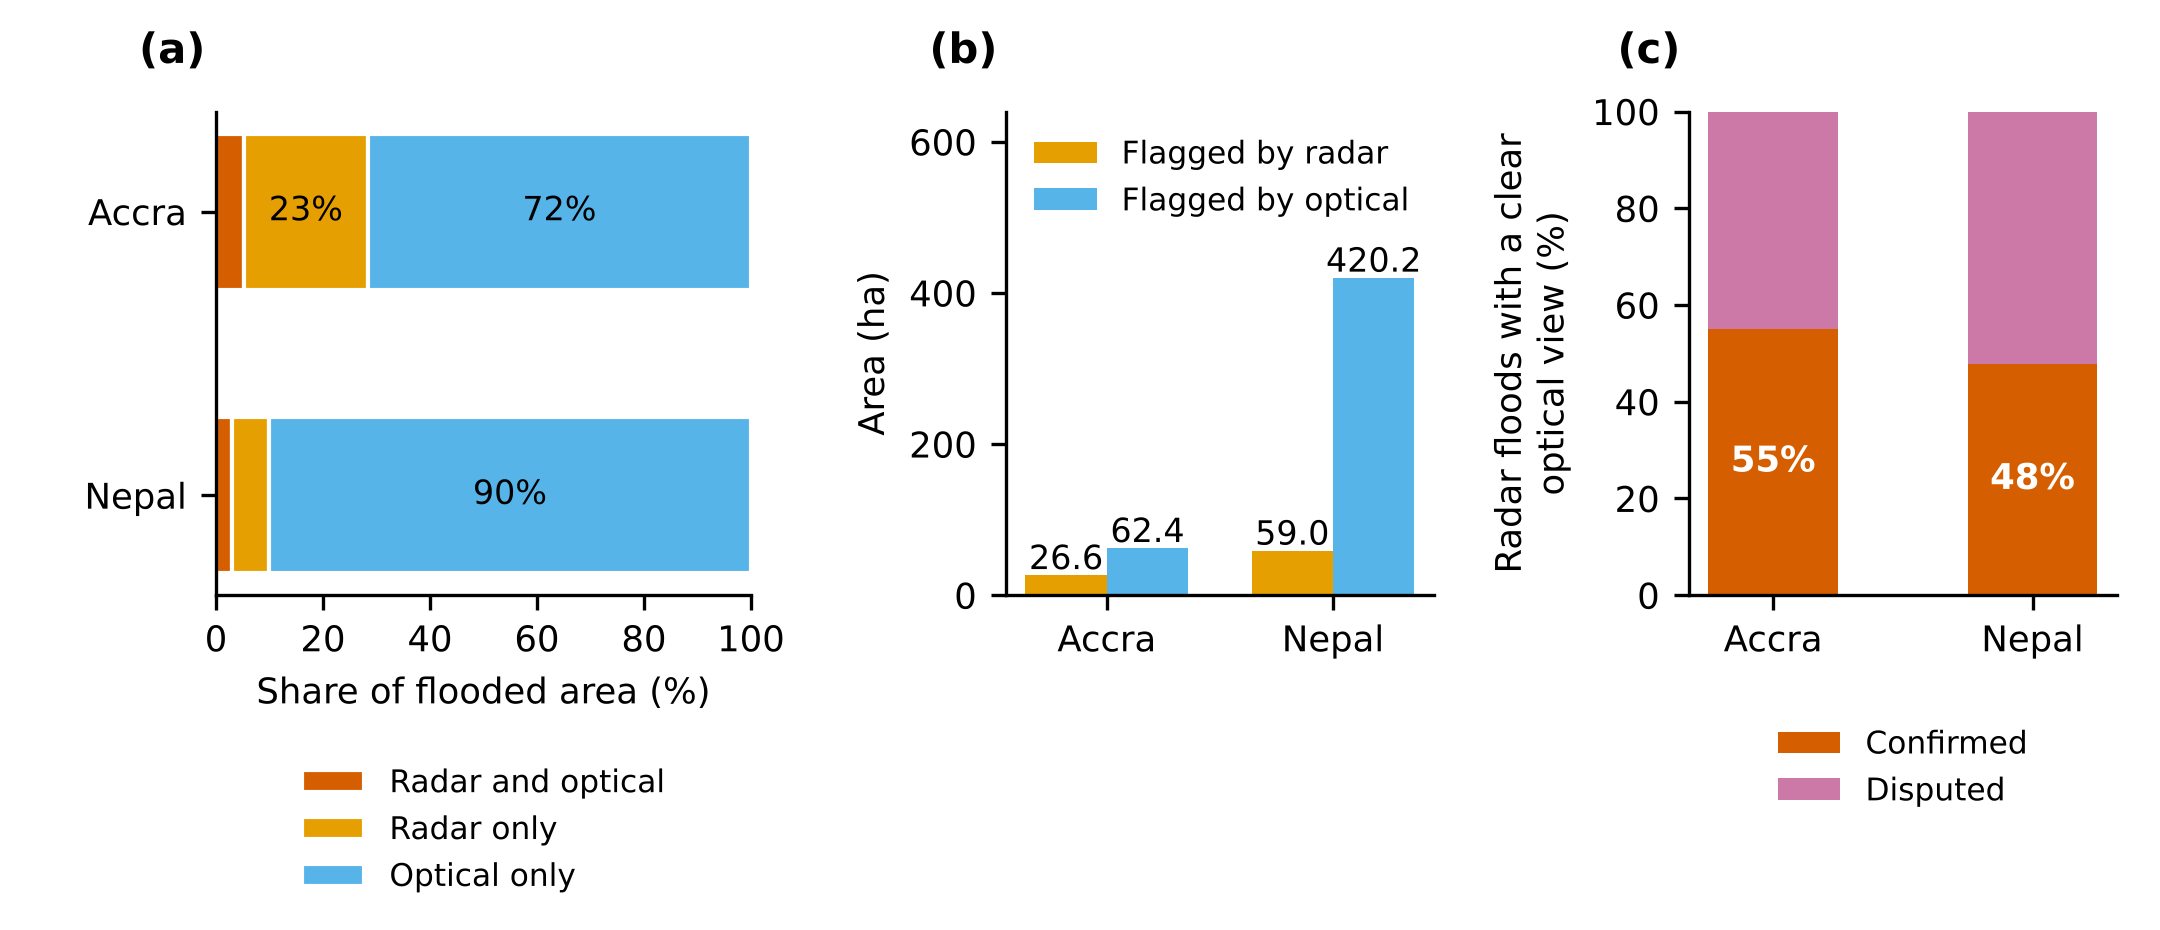
\includegraphics[width=\textwidth,height=9.2cm,keepaspectratio]{figs/fig_flood_classes.png}
\caption{Evidence classes of the two real flood runs. (a) Share of the flooded area by evidence class. (b) Area flagged by each sensor. (c) Fate of radar-flagged pixels that a clear optical view could check.}
\end{figure*}

\textit{Snow.} The pipeline mapped 93,272.0 ha as snow or ice in 1,023 km$^{2}$, 97.6\% of the valid area, with the NDSI threshold of 0.4 that defines the MODIS product \cite{hall1995ndsi}. The report prints one Sentinel-2 scene, a valid share of 93.4\% and its limitation that cloud and snow can look alike in some bands. The published evaluation concerns the daily MODIS product against stations in Austria \cite{tong2020snow}; it supports the method, not this scene, and no station was compared.

\textit{Two products in one box.} The land-cover pipeline gave 124.7 ha of permanent water (6.5\% of the 19.3 km$^{2}$ box) from WorldCover 2021, while the water-bodies pipeline gave 66.9 ha (3.5\%) at its default threshold of 0.3 in June 2024 (Fig. 8). The mask therefore holds 54\% of the area of the land-cover product. The report states that 0.3 is conservative and that the original cut is 0 \cite{mcfeeters1996ndwi}; the run was not repeated at 0, the two products differ in year and in sensor date, and we did not test why they differ.

\begin{figure}[!t]
\centering
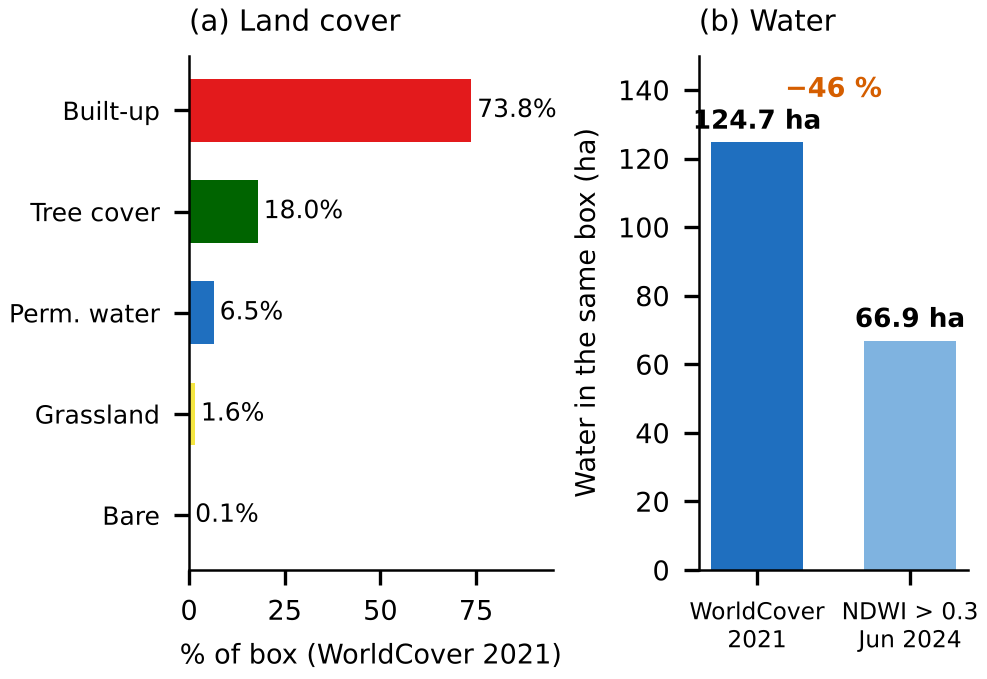
\includegraphics[width=\columnwidth,height=10.5cm,keepaspectratio]{figs/fig_london.png}
\caption{Land cover and water, two pipelines in the same London box. (a) Class shares from the land-cover run. (b) Water area from the land-cover run (WorldCover 2021) and from the water-bodies run (NDWI above 0.3, June 2024), both for the box $-$0.15 to $-$0.10, 51.47 to 51.52.}
\end{figure}

The answer to RQ3 is that the two flood runs and the Mexico City run agree with the outside world in time or in direction, the snow method agrees with its published evaluation, and a second product in London shows a 46\% difference that has a documented candidate cause; none of this is an accuracy measurement.

\subsection{RQ4: Transparency}

All 14 reports (14 of 14; exact 95\% interval 77\% to 100\%) contain a limitations section, a references list and a run record; 10 print the valid share with its denominator, and the other four describe published maps or datasets, for which it is not defined. Two automatic warnings fired: the coastal run printed that only 2\% of the area had cloud-free pixels (valid share 1.7\%) and the vegetation run printed the same for 44\%. In the Nepal run the report made three failures visible, the skipped terrain stage, the default threshold and the single optical scene. In the burn-severity run the report counted 49,568.1 ha as burned from dNBR of at least 0.10 on 15.6\% of the valid area with a mean of $-$0.023, and told the reader to choose dates close to the fire and in the same season; the run named no fire and used no perimeter, and we did not check whether a fire occurred.

One failure was not flagged. The radar-only flood run for Greater Accra reported 0.0 ha of flooding, a flooded share of 0.0\%, and a backscatter change of 0.000 dB at every percentile, and printed the same dates (4--16 June 2026) for the reference and the flood window, with four scenes in each. The report did not say that the two windows were identical. This is exactly the case that screening criterion C2 excludes, and it is the clearest gap in the reports we examined: a change analysis whose windows coincide should refuse or warn. Table VI lists what the reports exposed and what they did not.

\begin{table*}[!t]
\caption{Limits that the reports exposed, and one they did not}
\centering
{\footnotesize\setlength{\tabcolsep}{2.5pt}\renewcommand{\arraystretch}{1.12}\setlength{\tabw}{\dimexpr\textwidth-8\tabcolsep\relax}
\begin{tabular}{>{\raggedright\arraybackslash}p{\dimexpr0.1400\tabw\relax}>{\raggedright\arraybackslash}p{\dimexpr0.3000\tabw\relax}>{\raggedright\arraybackslash}p{\dimexpr0.3000\tabw\relax}>{\raggedright\arraybackslash}p{\dimexpr0.2600\tabw\relax}}
\toprule
\textbf{Run} & \textbf{Limit} & \textbf{Mechanism} & \textbf{How it became visible} \\
\midrule
Flood, Accra & Only 5\% of the flooded area confirmed by both sensors & Optical view clear over 18.1\% of the land & Valid optical share; class table \\
Flood, Nepal & Terrain stage not run & 13.5 million cells against a limit of 6 million & Applied flag, 0.0 ha removed \\
Flood, Nepal & Radar threshold not calibrated & Conventional $-$15.0 dB default; Otsu $-$7.1 dB & Threshold source printed \\
Flood, Nepal & 90\% of the flooded area optical only & One optical scene in the flood window & Class table; scene counts \\
Vegetation change & 44.2\% of the box valid & Cloud on one or both dates & Automatic warning \\
Coastal change & 1.7\% of the box valid & Cloud & Automatic warning; run excluded \\
Burn severity & Seasonal change can read as burn & Dates not close to a fire & Interpretation text \\
Water bodies & Mask smaller than a land-cover product & Conservative default threshold of 0.3 & Method text \\
Evapotranspiration & Model product, no uncertainty layer & Penman--Monteith from MODIS and reanalysis & Limitations text \\
Flood, radar only & Windows identical, zero change & Reference and flood scenes the same & Printed dates and zero statistics, not flagged \\
\bottomrule
\end{tabular}
}
\end{table*}

\section{Discussion and Conclusion}

\subsection{Answers to the Research Questions}

\textbf{RQ1.} On fourteen real runs the analyst listed one to five arguments (median 2.5) and received 10 to 17 files (median 13), including a report with its limitations. For flood mapping, a documented Earth Engine practice has 13 numbered steps and five auxiliary layers, against one statement and three arguments here. The comparison is documentary and the scope differs: the hosted practice needs no download and adds exposure analysis, whereas the local pipeline fuses two sensors, filters by terrain and reports evidence classes.

\textbf{RQ2.} PyGeoFetch registers 22 providers and implements parallel, resumable, checksum-verified downloads and a preflight gate, which the three access tools describe, in the pages read, only in part. On the Mexico City run the gate excluded 48 of 115 candidate scenes, about 360 GB or 42\% of the candidate volume, and the final velocity range was directionally consistent with a published peak.

\textbf{RQ3.} Both flood runs bracket a documented 2026 event, the snow run uses the threshold of the MODIS product whose published station agreement exceeds 97\%, and two products in one London box differ by 46\% in water area for a documented reason that was not tested.

\textbf{RQ4.} All 14 reports carry limitations and a run record (exact interval 77\% to 100\%); two warned automatically; the Nepal report exposed a skipped stage, a default threshold and a single optical scene; one failure, identical windows in a change analysis, was not flagged.

\subsection{Interpretation}

The stack lowers the effort to a first result by moving the decisions that analysts usually take by hand into defaults that are printed in the report. The two refusals and the no-data rule matter more than the call itself: a run that cannot be trusted stops or says so. The effort figures are counts, however. They do not show that a run is faster, and the downloads that PyGeoFetch performs have a cost in bandwidth that a hosted platform does not. PyGeoFetch's preflight gate is where that cost is reduced: on the one real run documented, it kept 42\% of the candidate volume off the network.

The flood runs show what the evidence classes are for. The reader of the Accra map can see that 72\% of the 81.4 ha rest on optical imagery alone and that optical imagery was clear over 18\% of the land; the reader of the Nepal map can see 90\% optical only, a skipped terrain stage and a default threshold, in a run whose window contains a flash flood of a kind (a debris-laden outburst in a narrow valley) that radar and 10 to 20 m optical water indices may handle poorly. We cannot say from these runs whether the optical-only class is mostly flood or mostly false water; the report prints it, which is the point, and the validation program of Table VIII would measure it. An urban pluvial flood such as Accra's is also the case that the report itself lists as under-mapped by radar.

The London comparison is a useful pattern: two pipelines on one box that disagree by 46\%, with a documented parameter as the candidate cause. A reader who has both reports can see the disagreement; a reader of one cannot. The failure of the radar-only run is the opposite pattern: the information was in the report (the dates) but nobody was told. The minimum indicators in Table VII follow from what the reports exposed, and from this failure. They are a proposal derived from fourteen runs, not a tested standard.

\begin{table*}[!t]
\caption{Proposed minimum set of reporting indicators, with the run that motivates each}
\centering
{\footnotesize\setlength{\tabcolsep}{2.5pt}\renewcommand{\arraystretch}{1.12}\setlength{\tabw}{\dimexpr\textwidth-6\tabcolsep\relax}
\begin{tabular}{>{\raggedright\arraybackslash}p{\dimexpr0.3200\tabw\relax}>{\raggedright\arraybackslash}p{\dimexpr0.3600\tabw\relax}>{\raggedright\arraybackslash}p{\dimexpr0.3200\tabw\relax}}
\toprule
\textbf{Indicator} & \textbf{What it prevents} & \textbf{Motivating run} \\
\midrule
Valid share, with the denominator named & A share of the valid area read as a share of the box & Vegetation (44.2\% valid) \\
No data kept out of every class & Cloud read as dry & Accra (optical clear 18.1\%) \\
Independent evidence per class & One sensor's claim read as confirmed & Nepal (90\% optical only) \\
Skipped stages and the reason & A filter assumed to have run & Nepal (terrain stage) \\
Source of each parameter (user, default, calibrated) & A default read as a calibration & Nepal ($-$15.0 dB default) \\
Distinct windows in a change analysis & Zero change read as no flood & Radar-only run (identical windows) \\
Agreement of products in one box & One product read as the truth & London (124.7 ha against 66.9 ha) \\
\bottomrule
\end{tabular}
}
\end{table*}

\subsection{Limitations}

Seven limitations qualify the findings. First, no result was compared with ground truth, so nothing here is an accuracy; the external agreement is of timing, direction and method. Second, the developer is also the evaluator: the author wrote the software, ran the analyses, selected the reports and chose the comparators, and the screening criteria were stated after the runs existed. Third, effort is measured by counts of arguments and files, not by time, and the comparator is a documented workflow, not a run; running time, bandwidth and memory were not recorded. Fourth, the Mexico City figures come from the author's own project documentation, were not re-run, and carry the inconsistencies that the documentation itself lists; a percentile range and a published peak are different statistics. Fifth, the comparison of access tools rests on the pages read, which describe some features only briefly. Sixth, the reports are from versions 2.1.8 to 2.2.0, their numbers were transcribed by hand, and the catalogue holds 41 pipelines in version 2.1.8; a later version may differ. Seventh, fourteen runs at a handful of places do not support inference to the other pipelines, and the object-based module and the foundation-model wrappers were not exercised.

\subsection{Future Work}

The next step is quantitative and independent. The Rasuwa event offers high-resolution post-event imagery under an open license \cite{roy2026nepalfloods} and a rapid-mapping activation \cite{cems2026emsr927}; the first test is whether the optical-only class of the Nepal run is flood or false water. A public benchmark of labelled flood chips \cite{bonafilia2020sen1floods11} gives a second test, and Table VIII lists the rest. A running-time and bandwidth benchmark against an access library and a hosted platform on the same box would turn the effort counts into measurements, and a check that refuses a change analysis with identical windows should be added to the pipelines.

\begin{table*}[!t]
\caption{Proposed validation program on real reference data (not yet run)}
\centering
{\footnotesize\setlength{\tabcolsep}{2.5pt}\renewcommand{\arraystretch}{1.12}\setlength{\tabw}{\dimexpr\textwidth-8\tabcolsep\relax}
\begin{tabular}{>{\raggedright\arraybackslash}p{\dimexpr0.1800\tabw\relax}>{\raggedright\arraybackslash}p{\dimexpr0.3200\tabw\relax}>{\raggedright\arraybackslash}p{\dimexpr0.3200\tabw\relax}>{\raggedright\arraybackslash}p{\dimexpr0.1800\tabw\relax}}
\toprule
\textbf{Question} & \textbf{Reference data} & \textbf{Measure} & \textbf{Related work} \\
\midrule
Is the optical-only flood class flood? & Post-event very-high-resolution imagery of Rasuwa, 27--28 Aug 2026 \cite{roy2026nepalfloods} & Share of class 3 pixels that are water on the reference & \cite{cems2026emsr927} \\
Flood extent against labels & Sen1Floods11 hand-labelled chips \cite{bonafilia2020sen1floods11} & IoU by evidence class, with and without the optical and terrain stages & \cite{twele2016flood,uddin2019bangladesh} \\
Snow cover & Climate stations and MODIS daily maps & Agreement of NDSI > 0.4 with stations on clear days & \cite{tong2020snow} \\
Water mask threshold & WorldCover and a national water layer & Water area against threshold, 0 to 0.3 & \cite{mcfeeters1996ndwi,zanaga2022worldcover} \\
InSAR velocity & Published rates for the same bowls & Velocity at common points & \cite{cigna2021mexico} \\
Time and bandwidth & The same flood question in Earth Engine or an access library & Wall-clock time, data volume, lines of code & \cite{gorelick2017gee,unspider2026flood} \\
\bottomrule
\end{tabular}
}
\end{table*}

\subsection{Conclusion}

An open, locally installed stack in which PyGeoFetch acquires and screens the data and PyGeoVision prepares, analyzes and reports takes a bounding box to a deliverable with a median of 2.5 arguments and returns a median of 13 files, including a report that states its limits. In fourteen real runs, its flood runs fall inside two documented 2026 events and show that most of the flooded area rests on one sensor; its preflight gate kept 42\% of a candidate InSAR download off the network; and its reports exposed most of their own limits, and missed one. These are findings about workflow and reporting. Accuracy against ground truth was not tested, and the validation program of Table VIII would show whether the numbers behind the indicators of Table VII are right.

\section*{Acknowledgment}

\textbf{Author contributions:} Conceptualization, methodology, software, investigation, formal analysis, visualization and writing: S. A. Kubi. \hl{[Co-author contributions to be completed by the author.]}

\textbf{Funding:} \hl{[Funding statement to be completed by the author; if there was none: ``This research received no external funding.'']}

\textbf{Data and code availability:} The source code of PyGeoVision (version 2.1.8) and PyGeoFetch (version 2.6.3) is public under the MIT license at \url{https://github.com/EOCoreINT/pygeovision} and \url{https://github.com/EOCoreINT/pygeofetch}. The 14 reports and the extracted numbers are supplied with the manuscript. \hl{[To be uploaded with the submission.]} The satellite data used (Copernicus Sentinel-1 and Sentinel-2, Copernicus DEM, ESA WorldCover, Microsoft building footprints, OpenStreetMap) are open.

\textbf{Acknowledgments:} Satellite data were provided free of charge through the Copernicus programme. The author used Claude (Anthropic) to read the reports, to check them against the repository and the installed packages, to verify references, and to draft and restructure the text, and has reviewed and edited the output and takes full responsibility for the content.

\textbf{Conflicts of interest:} The author develops and maintains the software evaluated in this paper. The author declares no other conflicts of interest.

\bibliographystyle{IEEEtran}
\bibliography{refs}

\end{document}
